% Created 2023-11-12 Sun 18:57
% Intended LaTeX compiler: pdflatex
\documentclass[12pt]{article}
\usepackage[utf8]{inputenc}
\usepackage[T1]{fontenc}
\usepackage{graphicx}
\usepackage{longtable}
\usepackage{wrapfig}
\usepackage{rotating}
\usepackage[normalem]{ulem}
\usepackage{amsmath}
\usepackage{amssymb}
\usepackage{capt-of}
\usepackage{hyperref}
\usepackage[utf8]{inputenc}
\usepackage{sbc-template}
\usepackage{graphicx,url}
\address{Universidade do Sul de Santa Catarina (UNISUL)\\ Tubarão - SC - Brasil\\ anajuliabit@gmail.com}
\usepackage[portuguese, brazilian]{babel}
\usepackage{biblatex}

\addbibresource{references.bib}
\author{Ana Julia Bittencourt Fogaça}
\date{\today}
\title{Análise de Bugs em Contratos Inteligentes de Blockchains Compatíveis com Ethereum Virtual Machine: Janeiro a Setembro de 2023}
\hypersetup{
 pdfauthor={Ana Julia Bittencourt Fogaça},
 pdftitle={Análise de Bugs em Contratos Inteligentes de Blockchains Compatíveis com Ethereum Virtual Machine: Janeiro a Setembro de 2023},
 pdfkeywords={},
 pdfsubject={},
 pdfcreator={Emacs 29.1 (Org mode 9.7)}, 
 pdflang={Portuges}}
\begin{document}

\maketitle

\section{Abstract}
\label{abstract}
\section{Resumo}
\label{resumo}
Software é criado por seres humanos e, consequentemente, está sujeito a bugs.
Isso não é diferente para aplicações que funcionam em blockchains que suportam a
Ethereum Virtual Machine (EVM). Entretanto, em contraste com software
convencional, as aplicações descentralizadas representam alvos particularmente
lucrativos para hackers, dada a natureza transparente e de código aberto da
blockchain. Neste artigo, analisamos 145 bugs descobertos durante auditorias
públicas em vários projetos desenvolvidos em Solidity, operando na Ethereum ou
em blockchains compatíveis com a EVM.
\section{Introdução}
\label{sec:org10e050d}
Introduzida em 2008 pelo whitepaper do Bitcoin
\autocite{nakamotoBitcoinPeertoPeerElectronic}, a tecnologia blockchain é
reconhecida como um vetor de transformação em múltiplas indústrias
\autocite{TechnologyTippingPoints}. Suas características de segurança robusta,
transparência e rastreabilidade, juntamente com a natureza de código aberto,
contribuem para sua adoção em operações críticas de negócios. Até 2023, o uso
mais evidente da blockchain, o mercado de criptomoedas, atingiu um valor de
mercado superior a um trilhão de dólares
\autocite{CryptocurrencyStatistics20232023}. A aplicabilidade da blockchain vai
além das criptomoedas, influenciando áreas como finanças, gerenciamento do,
identidade, saúde e governança eleitoral \autocite{BlockchainAdoptionsMaritime}.

A inovação do Ethereum, lançada pelo seu \emph{whitepaper} em 2014, representou um
marco na evolução da blockchain. Ao contrário do Bitcoin, concebido como uma
moeda eletrônica \emph{peer-to-peer} \autocite{nakamotoBitcoinPeertoPeerElectronic}, o
Ethereum apresentou o conceito inovador de "contratos inteligentes"
\autocite{EthereumWhitepaper}. Esta funcionalidade ampliou o escopo da blockchain,
permitindo sua aplicação em novos domínios. A plataforma Ethereum se destaca
pela hospedagem de uma máquina virtual que executa códigos em linguagens
\emph{Turing-complete}. No entanto, sendo os contratos inteligentes criados por
humanos, eles não estão isentos de falhas. Em um ambiente de código aberto,
típico de blockchains como Ethereum, essas falhas podem se tornar alvos
atrativos para hackers. Apenas no primeiro trimestre de 2023, ataques à rede
Ethereum resultaram no roubo de 320 milhões de dólares \autocite{HereHowMuch}. Para
minimizar tais riscos, é prática comum realizar auditorias nos contratos
inteligentes antes de seu lançamento em ambiente de produção. As auditorias
podem ser privadas, conduzidas por empresas especializadas, ou públicas, através
de plataformas como Code4rena \autocite{Code4renaKeepingHigh} e Sherlock
\autocite{Sherlock}, onde participantes diversos podem identificar
vulnerabilidades, sendo recompensados individualmente ou em grupo pela
descoberta de bugs.

Desde 2020, projetos de blockchain que negligenciaram o processo de auditoria
sofreram comprometimentos financeiros da ordem de 3.69 bilhões de dólares,
enquanto que projetos auditados reportaram perdas de 1.3
bilhões\autocite{CompetitiveVsPrivate}, sugerindo que, embora as auditorias reduzam
a probabilidade de ataques bem-sucedidos, ainda há desafios na detecção
antecipada de vulnerabilidades. Com a demanda por contratos inteligentes
crescendo e uma projeção de aumento anual de 82,2\% de 2023 a 2030
\autocite{SmartContractsMarket}, é crucial entender e classificar as
vulnerabilidades emergentes. Neste estudo, examinamos uma amostra de 145 bugs
identificados em 31 competições de auditoria públicas realizadas entre janeiro e
setembro de 2023 em duas plataformas de renome, Sherlock \autocite{Sherlock} e
Code4rena \autocite{Code4renaKeepingHigh}. Nosso objetivo é elucidar questões
fundamentais como a complexidade na detecção de diferentes tipos de bugs, a
incidência de categorias específicas de bugs em variados protocolos e a
correlação entre vulnerabilidades exploradas por hackers e aquelas identificadas
em competições de auditoria.

O artigo está divivido em..
\section{Revisão bibliográfica}
\label{sec:org4df6e0c}
\subsection{Ethereum Blockchain}
\label{sec:org11ce4e0}
Ethereum, conforme delineado no whitepaper por Vitalik Buterin et al., é uma
plataforma descentralizada que permite a construção de aplicações financeiras em
cima de uma infraestrutura de blockchain\autocite{EthereumWhitepaper}. A blockchain
é um sistema de registro distribuído e imutável que mantém um registro contínuo
de transações ou dados em blocos ligados por criptografia. Esse design assegura
a integridade e a veracidade dos dados, resistindo a alterações retroativas.
\subsection{Contratos inteligentes}
\label{sec:org7db25f4}
Contratos inteligentes são programas que rodam na blockchain do Ethereum,
permitindo que as partes cumpram acordos sem a necessidade de um intermediário.
Uma vez implantados, os contratos inteligentes não podem ser alterados, o que
exige que o código seja verificado para potenciais vulnerabilidades antes do
lançamento. Eles são fundamentais para a finança descentralizada e têm bilhões
de dólares em valor atrelados a eles\autocite{JCPFreeFullText}.
\subsection{Ethereum Virtual Machine}
\label{sec:orge4a4c48}
A Ethereum Virtual Machine (EVM) é o ambiente de execução para contratos
inteligentes na Ethereum. Funciona como uma camada global que pode executar
código de contrato inteligente em um contexto
descentralizado\autocite{woodETHEREUMSECUREDECENTRALISED}. Isso possibilita que os
desenvolvedores criem aplicações que funcionam exatamente conforme programadas,
sem qualquer possibilidade de fraude ou interferência de terceiros. A EVM é
isolada, significando que o código executado dentro dela não tem acesso ao
sistema de arquivos da rede, a outros contratos inteligentes, ou a qualquer
recurso externo. Esse isolamento garante um alto nível de segurança no
ecossistema Ethereum.
\subsection{Solidity}
\label{sec:org6a0b026}
Solidity é uma linguagem de programação de alto nível para a implementação de
contratos inteligentes e é fortemente tipada, suporta herança, bibliotecas e
tipos de usuário complexos\autocite{SoliditySolidity22}. Projetada para se alinhar
com a EVM, Solidity facilita o desenvolvimento de contratos inteligentes através
de uma sintaxe semelhante a JavaScript, tornando-a acessível a um amplo espectro
de programadores. Solidity, apesar de ser uma linguagem de alto nível com
características robustas, não está isenta de vulnerabilidades. Muitas delas
decorrem de uma desconexão entre a semântica da linguagem e a intuição dos
programadores, principalmente porque Solidity implementa características de
linguagens conhecidas, como JavaScript, de maneiras peculiares. Além disso, a
linguagem carece de construções específicas para lidar com aspectos do domínio
de blockchain, como a imprevisibilidade na ordem ou no atraso das etapas de
computação registradas publicamente na blockchain. Isso ressalta a importância
de uma compreensão aprofundada de Solidity ao desenvolver contratos
inteligentes, para mitigar o risco de vulnerabilidades de segurança.
\subsection{Finanças descentralizadas}
\label{sec:orgd82af0f}
Finanças Descentralizadas (DeFi) representam uma infraestrutura financeira
alternativa construída sobre a tecnologia blockchain, utilizando contratos
inteligentes para replicar serviços financeiros existentes de forma mais aberta,
interoperável e transparente\autocite{scharDecentralizedFinanceBlockchain}​​. DeFi é
uma evolução tecnológica emergente que vem ganhando destaque juntamente com
FinTech, RegTech, criptomoedas e ativos digitais, embora seu significado
completo, implicações legais e consequências políticas ainda sejam pouco
compreendidos​​. Este movimento revolucionário visa criar um sistema financeiro
baseado apenas em código, sem intermediários, e viu um crescimento de ativos
bloqueados de \$4 bilhões para \$104 bilhões em três
anos\autocite{meyerDecentralizedFinanceSystematic2022}​​. Ainda é uma área complexa
que exige uma compreensão rigorosa de suas nuances tanto por praticantes quanto
por pesquisadores de sistemas de
informação\autocite{gramlichMultivocalLiteratureReview2023}​​. Como um novo setor de
tecnologia financeira, DeFi tem o potencial de remodelar a estrutura da finança
moderna e criar um novo cenário para empreendedorismo e inovação, prometendo e
enfrentando desafios e limites​​\autocite{chenBlockchainDisruptionDecentralized2020}.
\subsection{Python}
\label{sec:org98a30f8}
\section{Metodologia e perguntas da pesquisa}
\label{sec:org908a3f9}
\subsection{Categoria dos protocolos}
\label{sec:orgbb946d6}
Os protocolos investigados neste estudo são dedicados ao setor de Finanças
Descentralizadas (DeFi), abarcando exclusivamente as seguintes subcategorias
conforme a classificação proposta por DefiLlama \autocite{DefiLlama}:

\begin{itemize}
\item Derivativos: Protocolos que disponibilizam ferramentas para operações
financeiras alavancadas, possibilitando que os usuários façam previsões e
especulações acerca de valores futuros de ativos, amplificando suas projeções
de lucro ou prejuízo.
\item Yield Farming: Protocolos que incentivam a prática de staking ou fornecimento
de liquidez por parte dos usuários, oferecendo recompensas por tais
atividades.
\item Agregadores de Yield: Protocolos que otimizam os rendimentos por meio da
integração de diversas estratégias de \emph{yield farming}.
\item Opções: Protocolos que ofertam o direito, embora não a obrigação, de adquirir
um ativo por um valor preestabelecido em um momento futuro.
\item DAOs (Organizações Autônomas Descentralizadas): Entidades organizacionais
inovadoras que operam sem centralização, com decisões sendo tomadas de forma
coletiva pelos membros.
\item Launchpads: Protocolos desenvolvidos para lançar novos projetos e criptoativos
no mercado.
\item Índices: Protocolos que rastreiam ou replicam a performance de uma série de
ativos interligados.
\item DEXs (Trocas Descentralizadas): Protocolos que permitem a troca de
criptoativos de forma descentralizada.
\item RWAs (Ativos do Mundo Real): Protocolos relacionados à tokenização de ativos
físicos, como imóveis.
\item Stablecoins: Criptomoedas com valor atrelado a moedas fiduciárias ou outros
ativos, buscando manter sua estabilidade por intermédio de mecanismos
descentralizados.
\item Gestores de Liquidez: Protocolos que gerenciam posições de liquidez em
formadores de mercado automatizados com liquidez concentrada.
\item Empréstimos: Protocolos que permitem o empréstimo e a tomada de empréstimos de
diversos ativos.
\end{itemize}
\subsection{Classificação dos Bugs}
\label{sec:org1ba8f1d}
A classificação das vulnerabilidades dos protocolos analisados neste trabalho
segue uma taxonomia híbrida, combinando os modelos propostos por Zhang et al.
\autocite{zhangDemystifyingExploitableBugs2023a} e as tags de Solodit
\autocite{Solodit_contentReport_tagsMd}, detalhada da seguinte forma:

\begin{itemize}
\item O: Fora do Escopo
\begin{itemize}
\item Inacessibilidade ao código-fonte do projeto.
\item Bugs manifestados em componentes off-chain.
\item Contratos inteligentes desenvolvidos em linguagens distintas
\end{itemize}
\item C01: Manipulação do Mempool / Vulnerabilidades de Front-Running
\begin{itemize}
\item Ataques do tipo sandwich \#TODO
\item Exploração baseado em \emph{Flash loans} \#TODO
\end{itemize}
\item C02: Ataque de Reentrada Vulnerabilidades de reentrância, resultantes de
chamadas externas realizadas antes da conclusão de atualizações de estado
internas, possibilitando a um adversário explorar o estado inconsistente.
\item C03: Atualizações de Estado Errôneas. Ausência ou incorreção na atualização de
estado, tal como uma atualização que não deveria ser efetuada.
\item C04: Configuração \emph{Hardcoded} Inserção de valores ou parâmetros estáticos
diretamente no código do contrato inteligente, o que pode representar um risco
de segurança se houver necessidade de flexibilidade.
\item C05: Escalada de Privilégios e Problemas de Controle de Acesso.
\begin{itemize}
\item Chamada de funções privilegiadas sem restrições adequadas.
\item Fundos de usuários que podem ser imobilizados por falhas ou ausência de
código de retirada.
\end{itemize}
\item C06: Matemática Incorreta / Contabilidade Errônea. Erros de cálculo
decorrentes de implementações matemáticas falhas, conduzindo a resultados
imprecisos, incluindo:
\begin{itemize}
\item Ordem incorreta de operações.
\item Retorno de valores inesperados.
\item Utilização de números incorretos para cálculos.
\item Erros de contabilidade.
\item Underflow/overflow.
\end{itemize}
\item C07: Lógica de Negócios Quebrada. Defeitos na lógica de negócios ou protocolos
que, mesmo alinhados à intenção do desenvolvedor, são inerentemente falhos.
\begin{itemize}
\item Invocações de funções inesperadas ou omissas
\item Condições anômalas de ambiente ou contrato
\item Argumentos de função impróprios
\end{itemize}
\item C08: Bugs Específicos da Implementação do Contrato. Bugs que não se enquadram
claramente em outras categorias.
\item C09: Falta de Proteção Contra Replay de Assinatura
\begin{itemize}
\item Nonce ausente \#TODO
\item Colisão de hash.
\end{itemize}
\item C10: Verificação Ausente. Omissão crítica de condições ou validações
essenciais no código.
\item C11: DoS (Negação de Serviço). Vulnerabilidades que permitem a um atacante
comprometer a resposta ou eficiência do contrato. Esta categoria inclui casos
que não são bem descritos por outra classe e onde a consequência primária é o
encerramento do contrato ou ineficiência operacional.
\item C12: Validação de Dados Falhas na verificação ou saneamento de entradas,
particularmente daquelas oriundas de fontes externas.
\item C13: Correspondência de Lista Branca/Lista Negra. Gerenciamento inadequado de
endereços baseado em listas predefinidas.
\item C14: Arrays. Vulnerabilidades associadas ao manuseio inadequado de arrays,
incluindo:
\begin{itemize}
\item Leituras/escritas fora dos limites
\item Problemas na exclusão
\item Questões relacionadas ao redimensionamento de arrays
\end{itemize}
\end{itemize}
\subsection{Coleta de dados}
\label{sec:org70481ef}
\begin{table}[htbp]
\caption{\label{TABELA1}Visão Geral das Competições Avaliadas. 'HRF' (High Risk Findings) representa bugs de alta severidade. 'nSLOC' indica o número total de linhas de código associadas a cada competição.}
\centering
\begin{tabular}{lllrrrrr}
Plataforma & Categoria & Competição & Prêmio & HRF & nSLOC & Participantes & Data\\[0pt]
\hline
Code4rena & DAO & \href{https://code4rena.com/reports/2023-08-arbitrum}{Arbitrum security council election} & 90500 & 1 & 2184 & 39 & 2023-09\\[0pt]
Code4rena & DAO & \href{https://code4rena.com/reports/2023-06-llama}{Llama} & 60500 & 2 & 2096 & 50 & 2023-07\\[0pt]
Code4rena & Stablecoin & \href{https://code4rena.com/reports/2023-06-lybra}{Lybra finance} & 60500 & 8 & 1762 & 136 & 2023-08\\[0pt]
Code4rena & Dexes & \href{https://code4rena.com/reports/2023-05-maia}{Maia DAO ecosystem} & 300500 & 35 & 10997 & 85 & 2023-05\\[0pt]
Code4rena & Yield & \href{https://code4rena.com/reports/2023-07-pooltogether\#wardens}{PoolTogether} & 121650 & 9 & 3324 & 117 & 2023-07\\[0pt]
Code4rena & Yield & \href{https://code4rena.com/reports/2023-08-pooltogether}{PoolTogether v5: part deux} & 42000 & 2 & 1001 & 45 & 2023-08\\[0pt]
Sherlock & Lending & \href{https://audits.sherlock.xyz/contests/75}{Ajna update} & 85600 & 6 & 5659 & 155 & 2023-06\\[0pt]
Sherlock & Yield Agreggator & \href{https://audits.sherlock.xyz/contests/41}{Blueberry} & 72500 & 10 &  & 284 & 2023-02\\[0pt]
Sherlock & Yield Agreggator & \href{https://audits.sherlock.xyz/contests/104/report}{Blueberry Update \#3} & 23600 & 5 & 3633 & 183 & 2023-08\\[0pt]
Sherlock & Opções & \href{https://audits.sherlock.xyz/contests/99}{Bond options} & 23600 & 2 & 885 & 153 & 2023-07\\[0pt]
Sherlock & Empréstimos & \href{https://audits.sherlock.xyz/contests/107}{Cooler update} & 17000 & 4 & 512 & 170 & 2023-08\\[0pt]
Sherlock & Dexes & \href{https://audits.sherlock.xyz/contests/97}{GFX labs} & 20400 & 2 & 716 & 106 & 2023-07\\[0pt]
Sherlock & Derivativos & \href{https://audits.sherlock.xyz/contests/74}{GMX} & 200000 & 5 & 10571 & 220 & 2023-04\\[0pt]
Sherlock & Lending & \href{https://audits.sherlock.xyz/contests/84}{Iron bank} & 67400 & 1 & 2241 & 271 & 2023-05\\[0pt]
Sherlock & Derivativos & \href{https://audits.sherlock.xyz/contests/79}{Perennial} & 122000 & 1 & 4063 & 220 & 2023-05\\[0pt]
Sherlock & Derivativos & \href{https://audits.sherlock.xyz/contests/106}{Perennial v2} & 125200 & 6 & 2494 & 252 & 2023-07\\[0pt]
Sherlock & Derivativos & \href{https://audits.sherlock.xyz/contests/85}{Symmetrical} & 91000 & 8 & 3553 & 233 & 2023-06\\[0pt]
Sherlock & Derivativos & \href{https://audits.sherlock.xyz/contests/108}{Symmetrical Update} & 27600 & 2 & 3921 & 52 & 2023-08\\[0pt]
Sherlock & Launchpad & \href{https://audits.sherlock.xyz/contests/100}{Tokensoft} & 21400 & 1 & 769 & 221 & 2023-07\\[0pt]
Sherlock & Stablecoin & \href{https://audits.sherlock.xyz/contests/73}{Unitas protocol} & 36400 & 1 & 1433 & 208 & 2023-06\\[0pt]
Code4rena & RWA & \href{https://code4rena.com/contests/2023-01-ondo-finance-contest}{Ondo finance} & 60500 & 1 & 4365 & 74 & 2023-01\\[0pt]
Sherlock & Índices & \href{https://audits.sherlock.xyz/contests/81}{Index coop} & 130600 & 2 & 4383 & 283 & 2023-05\\[0pt]
Sherlock & Stablecoin & \href{https://audits.sherlock.xyz/contests/82}{USSD} & 18200 & 3 & 402 & 224 & 2023-05\\[0pt]
Sherlock & RWA & \href{https://audits.sherlock.xyz/contests/98}{Dinari} & 16000 & 1 & 575 & 176 & 2023-07\\[0pt]
Sherlock & Dexes & \href{https://audits.sherlock.xyz/contests/88}{RealWagmi} & 33200 & 5 & 1080 & 203 & 2023-06\\[0pt]
Code4rena & DAO & \href{https://code4rena.com/reports/2023-07-nounsdao}{Nouns DAO} & 100000 & 1 & 9098 & 36 & 2023-07\\[0pt]
Sherlock & Dexes & \href{https://audits.sherlock.xyz/contests/89}{DODO v3} & 57800 & 5 & 2079 & 151 & 2023-06\\[0pt]
Sherlock & Derivativos & \href{https://audits.sherlock.xyz/contests/72}{Hubble Exchange} & 60000 & 3 & 1945 & 148 & 2023-06\\[0pt]
Code4rena & Stablecoin & \href{https://code4rena.com/contests/2023-06-angle-protocol-invitational}{Angle Protocol} & 52500 & 3 & 2276 & 5 & 2023-07\\[0pt]
Code4rena & Gestores de liquidez & \href{https://audits.sherlock.xyz/contests/86}{Arrakis} & 81400 & 2 & 2801 & 247 & 2023-06\\[0pt]
Sherlock & Dexes & \href{https://audits.sherlock.xyz/contests/95}{Unstoppable} & 36400 & 8 & 2035 & 130 & 2023-06\\[0pt]
\hline
TOTALS &  &  & 2255950 & 145 & 3095.1 & 157.32258 & \\[0pt]
\end{tabular}
\end{table}

No período de janeiro a setembro de 2023, nossa análise focou em 31 das competições de auditoria pública realizadas nas plataformas Code4rena \autocite{Code4renaKeepingHigh} e Sherlock \autocite{timeMostInterestingWeb32023}, nas quais foram identificados 145 bugs de alta severidade. Com duração média de sete dias, estes eventos visaram a identificação de falhas críticas em contratos inteligentes antes de seu lançamento final. A \hyperref[TABELA1]{Tabela 1} detalha as competições examinadas, incluindo o número de participantes, o prêmio total, a categoria do projeto, a quantidade de vulnerabilidades de alta severidade encontradas e o total de linhas de código abrangidas em cada competição. O valor total das recompensas distribuídas nesses eventos superou os dois milhões de dólares, com uma média de 150 participantes por evento. Após a fase de submissão, juízes especializados em auditoria de contratos inteligentes, selecionados pela comunidade, avaliaram a severidade dos bugs. Os bugs classificados como de alta severidade representam riscos significativos, incluindo a possibilidade de roubo ou perda de ativos digitais \autocite{JudgingCriteria}. Todos os bugs, suas descrições e a classificação realizada estão disponíveis no nosso dataset \autocite{bittencourtSolidityCommonVulnerabilities2023}
\subsection{Perguntas da pesquisa}
\label{sec:org31a0553}
Nos focamos nas seguintes perguntas de pesquisa:
\begin{itemize}
\item Q1: Que tipo de vulnerabilidade é mais difícil de ser encontrada por
auditores?
\item Q2: Que categoria de protocolo apresenta mais presença de bugs?
\item Q3: Os auditores frequentemente perdem tipos específicos de bugs que são
posteriormente explorados?
\item Q4: Qual é o impacto financeiro médio de diferentes tipos de vulnerabilidades?
\item Q5: Como a complexidade do contrato inteligente afeta a probabilidade de
encontrar bugs?
\item Q6: Qual a relação entre categoria de bugs e os diferente tipos de protocolos?
\end{itemize}
\section{Análise e Discussão dos Resultados}
\label{sec:orga6428ea}
\subsection{Análise de dados coletados}
\label{sec:org0697a7a}
A identificação de vulnerabilidades em contratos inteligentes é uma tarefa que
exige extrema atenção aos detalhes e uma mentalidade orientada para a descoberta
de falhas, similar à de um potencial atacante. Nesse cenário, os auditores
enfrentam desafios significativos na condução de suas investigações,
principalmente porque muitos bugs ainda passam despercebidos
\autocite{CompetitiveVsPrivate}. Para aprofundar nosso entendimento desses
desafios, realizamos uma análise exploratória do , utilizando as bibliotecas
Python Panda e Seaborn. O script empregado nessa análise está documentado em
\autocite{bittencourtsoliditycommonvulnerabilities2023}, e todos os gráficos nesta
seção foram gerados a partir dele.

As principais descobertas da nossa análise incluem:

\begin{enumerate}
\item A detecção de bugs por um número limitado de auditores indica uma complexidade elevada na sua identificação. Como ilustrado na Figura 1, entre as diversas categorias de vulnerabilidades, aquelas associadas a Falhas Específicas na Implementação de Contratos (C08), seguidas pelas Vulnerabilidades de Reentrância (C02) e a Ausência de Verificações (C10), emergem como as mais desafiadoras de serem detectadas. Em contraste, as categorias como Problemas de Controle de Acesso e Escalada de Privilégios (C05), Arrays (C14), e Manipulação de Mempool / Vulnerabilidades de Front-Running (C01) são relativamente mais fáceis de serem identificadas.
\end{enumerate}

\begin{figure}[h]
  \centering
  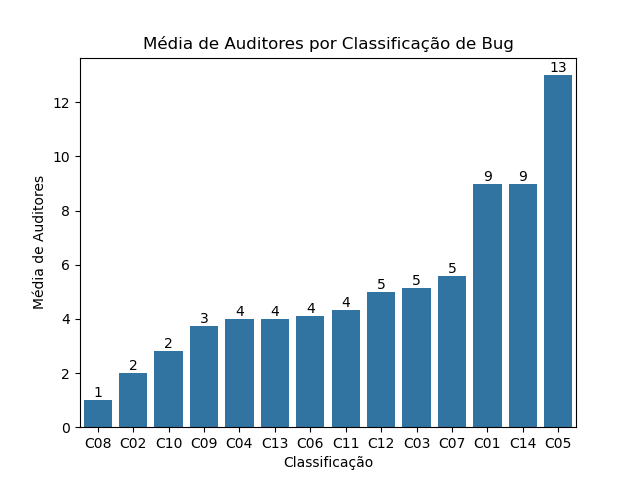
\includegraphics[width=\linewidth]{../results/average_auditors_by_class.png}
  \caption{Média de auditores por classificação}

  \label{fig:grafico_1}
\end{figure}


\begin{enumerate}
\item C06 - Erros de Cálculo (Matemática Incorreta/Contabilidade Errônea): De acordo com a Figura 2, podemos notar que esta categoria é a mais prevalente, indicando que falhas em lógica matemática, como underflows/overflows ou sequências errôneas de operações, são desafios comuns no setor de Finanças Descentralizadas (DeFi). Isso é compreensível, considerando que o DeFi opera intensamente com cálculos matemáticos complexos. Esta observação implica que numerosos contratos inteligentes são vulneráveis devido a implementações falhas de operações matemáticas, potencialmente resultando em perdas financeiras substanciais.

\begin{figure}[h]
  \centering
  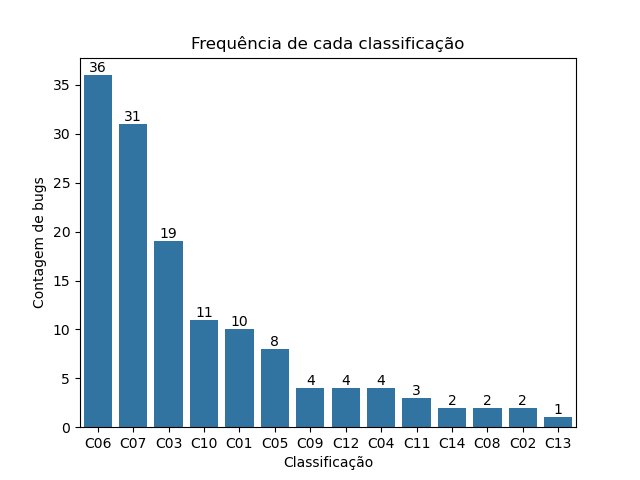
\includegraphics[width=\linewidth]{../results/bugs_by_class.png}
  \caption{Frequncia de bugs por classificação}

  \label{fig:grafico_2}
\end{figure}
\end{enumerate}


\begin{enumerate}
\item C07 - Lógica de Negócios Quebrada: A segunda classificação mais comum conforme mostra a Figura 2, mostrando que muitos contratos têm falhas inerentes na lógica de negócios, que poderiam ser prevenidas com uma análise e teste mais detalhados das regras de negócio e cenários de contrato.

\item C03 - Atualizações de Estado Errôneas: A terceira classificação em frequência sugere que uma quantidade considerável de contratos tem falhas na lógica que gerencia o estado do contrato, o que pode levar a consequências imprevistas e possíveis vulnerabilidades de segurança.

\item Classes Menos Frequentes (C02, C08, C13): Vulnerabilidades como Reentrância (C02) e Falhas Específicas na Implementação de Contratos (C08) são menos frequentes, o que pode ser interpretado como um sinal de que são mais difíceis de detectar, o que condiz com a nossa descoberta 1 de que C02 e C08 são as categorias mais difíceis de serem identificadas. A classe C13, que inclui vulnerabilidades como o uso de funções de hash inseguras, também é menos frequente, o que pode indicar que os desenvolvedores estão mais conscientes dessas vulnerabilidades e as evitam.

\item C01 - Manipulação de Mempool/Vulnerabilidades de Front-Running: Apesar de menos comuns, estas vulnerabilidades podem ter impactos devastadores, permitindo ataques de 'sandwich' ou exploração baseada em empréstimos instantâneos ('flash loans'), destacando a necessidade de estratégias de mitigação robustas.
\end{enumerate}

Vulnerabilidades de Implementação Específica (C08) e Proteção Contra Replay (C09): São menos comuns, o que pode sugerir que são específicas de certos contratos ou que a conscientização e ferramentas de detecção para essas vulnerabilidades são eficazes.

C14 - Arrays: Menos frequente, mas ainda assim significativa, essa categoria indica problemas no manuseio de arrays, como leituras/escritas fora dos limites, que são bugs mais técnicos e possivelmente menos explorados em ataques reais.

Classes dominantes de vulnerabilidades, como atualizações de estado incorretas (C03), problemas de controle de acesso e escalada de privilégios (C05), e erros de cálculo (C06), são recorrentes em várias categorias. Esses padrões indicam a prevalência desses tipos de vulnerabilidades.

Algumas classes de vulnerabilidades são menos frequentes, sugerindo especificidade para certos tipos de protocolos ou maior dificuldade na detecção, como é o caso da falta de proteção contra replay de assinaturas (C09), ausência de verificações (C10) e bugs específicos de implementação de contrato (C08).

As diferentes categorias de protocolo apresentam distintos perfis de vulnerabilidade. Por exemplo, protocolos Dexes apresentaram o maior número de bugs identificados.

Há uma correlação complexa entre as categorias de vulnerabilidade e os diferentes tipos de protocolos, com variações significativas nas classificações mais frequentes entre as categorias."

\begin{itemize}
\item Bugs cujo foram identificados por uma quantidade menor de
auditores, indicam uma maior dificuldade na identificação dos mesmos. Dos
vários tipos de vulnerabilidades, aqueles relacionados a bugs específicos da
implementação do contrato (C8), seguidos por Ataque de Reentrada
Vulnerabilidades de reentrância (C02) e Verificação Ausente (C10), são
particularmente difíceis de identificar. Inversamente, C05, C14 e C01 são os
mais fáceis de identificar.
\item Atualizações de estado errôneas (C03), escalada de privilégios e problemas de
controle de acesso (C05) e cálculos errados (C06) são as classes dominantes de
vulnerabilidades em várias categorias. Isso sugere que esses tipos de
vulnerabilidade são comuns em geral. Especificamente, atualizações de estado
errôneas são encontradas em oito categorias, enquanto escalada de privilégios
e problemas de controle de acesso (C05) e cálculos errados (C06) aparecem em
sete categorias.
\item Certas classes de vulnerabilidades aparecem com menos frequência, indicando
que podem ser específicas para certos tipos de protocolo ou mais desafiadoras
de encontrar. Por exemplo, classes como falta de proteção contra replay de
assinatura (C09), checagem ausente (C10) e bugs específicos da implementação
de contrato (C08) são escassos.
\item Diferentes categorias de protocolo têm diferentes perfis de vulnerabilidade.
Protocolos Dexes tiveram o maior número de bugs identificados, com 47
classificados, seguidos por Derivativos com 25 e Agregador e Stablecoin com 15
cada.
\item Cálculos errados (C06) é a classificação mais frequente em todas as
categorias, com 36 bugs classificados dessa forma. Lógica de negócios quebrada
(C07) é a segunda classificação mais frequente, com 31 bugs identificados.
Atualizações de estado errôneas (C03) e checagem ausente (C10) seguem com 19 e
11 bugs classificados, respectivamente. Finalmente, 10 bugs foram
classificados como Manipulação de Mempool / Vulnerabilidades de Front-Running
(C01).
\item A relação entre categorias de vulnerabilidade e diferentes tipos de protocolo
é complexa. Cálculos errados (C06) é a classificação mais frequente encontrada
em Derivativos, Agregador de Rendimentos e Stablecoins, enquanto Lógica de
negócios quebrada (C07) é a classificação mais frequente encontrada em Dexes e
Rendimentos. Além disso, arrays (C14) e cálculos errados (C06) são o segundo
tipo mais comum de bugs encontrados em Dexes.
\end{itemize}
\subsection{Perguntas de pesquisa}
\label{sec:org779243e}
\begin{enumerate}
\item Por que Bugs Específicos da Implementação do Contrato (C08) São Mais
Desafiadores de Identificar? Esta pergunta visa explorar os fatores
subjacentes que tornam bugs específicos, particularmente C08 e C02, mais
difíceis de serem identificados por auditores.
\item O Que Torna Certas Vulnerabilidades Mais Fáceis de Detectar? Focando em
vulnerabilidades como C05, C14 e C01, esta pergunta busca entender as
características que as tornam mais aparentes para os auditores.
\item Vulnerabilidades Comuns Entre Categorias de Protocolo Indicam Problemas
Sistêmicos? Investigar por que atualizações de estado errôneas (C03),
escalada de privilégios (C05) e cálculos errados (C06) são comuns em várias
categorias pode revelar problemas sistêmicos mais amplos no design de
contratos inteligentes.
\item Quais Fatores Contribuem para a Raridade de Certas Classes de
Vulnerabilidade? Olhando para vulnerabilidades menos frequentes como C09, C10
e C08, esta pergunta investiga por que essas classes são menos comuns,
explorando se são específicas do protocolo ou inerentemente difíceis de
detectar.
\item Como Diferentes Categorias de Protocolo Influenciam o Perfil de
Vulnerabilidades? Esta pergunta visa entender a relação entre categorias de
protocolo (como Dexes, Derivativos
\end{enumerate}
\subsection{Resultados}
\label{sec:orga86b5ef}
\subsubsection{Q1: Que tipo de vulnerabilidade é mais difícil de ser encontrada por auditores?}
\label{sec:orgfe32f5a}
Em nossa análise sobre a dificuldade de detecção de vulnerabilidades por
auditores em contratos inteligentes, identificamos que as vulnerabilidades com
uma média menor de auditores envolvidos na detecção tendem a ser mais
desafiadoras. Especificamente, as categorias Específicos da Implementação do
Contrato (C08) e Ataque de Reentrada (C02) emergem como as mais complexas, com
médias de apenas 1 e 2 auditores, respectivamente. Isso indica que essas
vulnerabilidades podem ser mais sutis ou requerer uma expertise mais
especializada, o que as torna menos detectáveis em auditorias.

Contrastando, categorias como Escalada de Privilégios e Problemas de Controle de
Acesso (C05), com média de 13 auditores, Manipulação do Mempool /
Vulnerabilidades de Front-Running (C01) e Arrays (C14), ambas com média de 9
auditores, Lógica de Negócios Quebrada (C07), com média de aproximadamente 5.58
auditores, e Atualizações de Estado Errôneas (C03), com média de aproximadamente
5.16 auditores, demonstram ser mais facilmente detectáveis. Essas categorias
possivelmente são mais evidentes ou exigem menos especialização técnica para sua
identificação, culminando em uma frequência maior de detecção em auditorias.
Esta análise sublinha a necessidade de uma compreensão aprofundada das
diferentes classes de vulnerabilidades em contratos inteligentes e enfatiza o
papel crucial dos auditores especializados em sua identificação e mitigação.

\begin{itemize}
\item Q2: Que categoria de protocolo apresenta mais presença de bugs?
\item Q3: Os auditores frequentemente perdem tipos específicos de bugs que são
posteriormente explorados?
\item Q4: Qual é o impacto financeiro médio de diferentes tipos de vulnerabilidades?
\item Q5: Como a complexidade do contrato inteligente afeta a probabilidade de
encontrar bugs?
\item Q6: Qual a relação entre categoria de bugs e os diferente tipos de protocolos?
\end{itemize}
\section{Considerações finais}
\label{sec:org8d03d30}

\printbibliography
\end{document}